%%%%%%%%%%%%%%%%%%%%%%%%%%%%%%%%%%%%%%%%%%%%%%%%%%%%%%%%%%%%%%%%%%%%%%%%%%%%
%%%%%                          GLOSSAIRE                              %%%%%%
%%%%%%%%%%%%%%%%%%%%%%%%%%%%%%%%%%%%%%%%%%%%%%%%%%%%%%%%%%%%%%%%%%%%%%%%%%%%

\phantomsection 
\addcontentsline{toc}{chapter}{Glossary} \mtcaddchapter
\label{Ann:gloss}
\addtocontents{toc}{\protect\addvspace{10pt}}

\vspace*{-1.6cm}
\begin{flushright}
\section*{\fontsize{20pt}{20pt}\selectfont\textnormal{Glossary}}
\end{flushright}
\vspace{-0.2cm}


\lhead[\fancyplain{}{Glossary}]
      {\fancyplain{}{}}
\chead[\fancyplain{}{}]
      {\fancyplain{}{}}
\rhead[\fancyplain{}{}]
      {\fancyplain{}{Glossary}}
\lfoot[\fancyplain{}{}]
      {\fancyplain{}{}}
\cfoot[\fancyplain{}{\thepage}]
      {\fancyplain{}{\thepage}}
\rfoot[\fancyplain{}{}]%
     {\fancyplain{}{\scriptsize}}

%%%%%%%%%%%%%%%%%%%%%%%%%%%%%%%%%%%%%%%%%%%%%%%%%%%%%%%%%%%%%%%%%%%%%%%%%%
%%%%%                      Start part here                          %%%%%%
%%%%%%%%%%%%%%%%%%%%%%%%%%%%%%%%%%%%%%%%%%%%%%%%%%%%%%%%%%%%%%%%%%%%%%%%%%

\lettrine[lines=1]{S}{ }ome terms used along this thesis may lead to confusion to an uninitiated person, as they are closely related, but describe slightly different concepts. This glossary compares and clarifies them.

\vspace*{1cm}

\noindent\textbf{Markers vs. Keypoints}\\
Markers are objects attached to the body of the user, often small and round. They are used to indirectly track the posture of a user. Markers can sometimes be active and emit light, instead of passive and reflect light. They can also be anchored to the bone, for a more precise analysis exempt from Soft Tissue Artifact (STA). A marker-based analysis commonly refers to the use of passive markers, glued to the skin of the user.\\
Keypoints are points of interest detected by a machine learning model, either in 2D or in 3D space. They can estimate the location of a human joint, or of a body part, or else of any point of interest of any object.\\
Once triangulated, they can be treated like markers, for example while running inverse kinematic (IK) analysis.

\vspace*{0.5cm}

\noindent\textbf{Markerless vs. Sensorless}\\
Markerless systems don't use any markers, but they can use other sensors, such as Inertial Measurement Units (IMUs). \\
In contrast, sensorless systems don't involve any wearable markers nor any sensors. This also goes for sensorless dynamic analysis, which does not use any force sensors, or for muscle activation analysis, which does not use any Electromyography (EMG) sensor. \\
Note that approaches only using video (RGB), or depth-field video (RGB-D) sensors are usually considered sensorless, as they do not involve any particular alteration to the environment or behavior of the user.

\vspace*{0.5cm}

\noindent\textbf{Gold standard vs. Silver standard}\\
A gold-standard method refers to the best currently available method, usually in terms of accuracy, which can be used as a reference to compare other methods. \\
Marker-based methods cannot be rigorously considered as such, since they are sensitive to Soft Tissue Artifact (STA) and to positioning variability from the operator. In contrast, bone-anchored pins, Magnetic Resonance Imaging (MRI), biplanar videoradiography, or 3D ultrasounds are considered to be closer to a gold-standard. \\
However, the latter methods are not available for all activities worthy of scientific interest, and marker-based ones are often preferred. Therefore, they are considered as a silver-standard.\\
Nevertheless, the literature sometimes refer to them as gold-standard, as opposed to IMU or markerless systems, which are considered as silver-standard.

\vspace*{0.5cm}

\noindent\textbf{Silhouette vs. Shape}
morphology
vs. mesh (geometric representation of a shape)

\vspace*{0.5cm}

\noindent\textbf{Machine learning vs. Deep learning}\\
Machine learning and Deep Learning, as well as Artificial Intelligence, Artificial Neural Networks, or Convolutional Neural Networks, are sometimes used interchangeably. However, they do not exactly refer to the same concepts (Figure~\ref{fig_ai}).\\
Artificial Intelligence (AI) concerns the general concept of machines being able to perform tasks that would seem to require human intelligence, or even to sense, reason, and act accordingly. \\
Machine learning (ML) is a subset of AI, and refers to the concept of machines being able to learn and improve as they are exposed to data. It is a data-driven approach, as opposed to knowledge-driven ones.\\
Artificial Neural Networks (ANN) are a specific way of performing ML, by using a network of units inspired from the natural neuron, and thus mimicking the brain. Convolutional Neural Networks (CNN) are a type of ANN which is particularly suited for image processing.\\
Deep Learning (DL) refers to an ANN with more than 3 layers of neurons.

\begin{figure}[hbtp]
	\centering
            \def\svgwidth{1\columnwidth}
            \fontsize{10pt}{10pt}\selectfont
            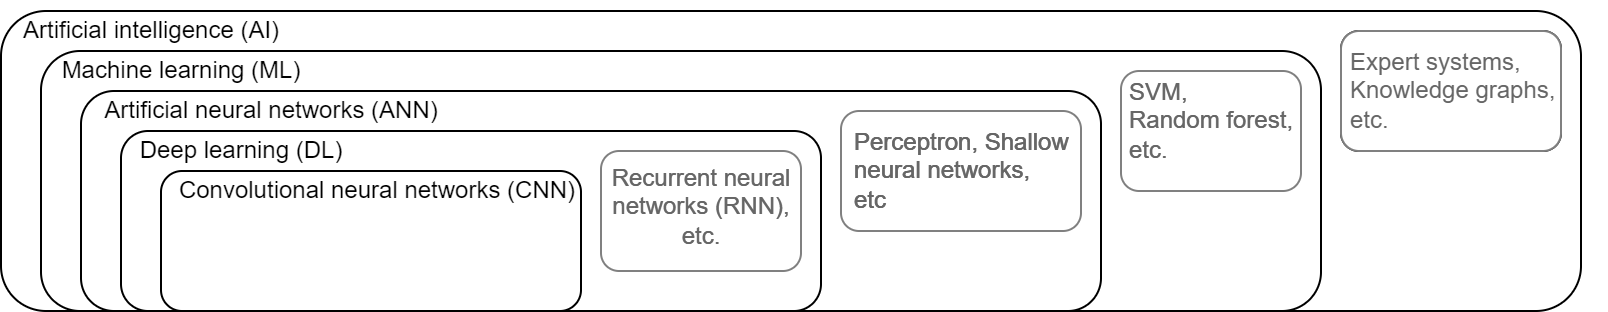
\includegraphics[width=\linewidth]{"../Annexes/Figures/AI_CNN_etc.png"}
            \caption{Diagram of Artificial intelligence, Machine learning, Artificial neural networks, Convolutional neural networks, and Deep learning. The greyed out elements will not be described.}
            \label{fig_ai}
\end{figure}

\vspace*{0.5cm}

\noindent\textbf{Kinematics vs. Kinetics }
vs dynamics

\vspace*{0.5cm}

\noindent\textbf{Spatio-temporal parameters vs Joint kinematics}
both fall under the umbrella of kinematic data. In the customary usage, kinematics describes joint kinematics.

\vspace*{0.5cm}

\noindent\textbf{Forward kinematics vs. Direct kinematics}
vs. inverse kinematics




% top-down vs. bottom-up
% Monocular/single view vs. Multiview: videos or images

